\documentclass[aspectratio=1610]{beamer}
\usetheme{metropolis} % Use the Metropolis theme
% \usepackage{xeCJK}
% \setCJKmainfont{SimSun}
\usepackage{multirow}
\usepackage{graphicx}
\usepackage{booktabs} % for better table formatting
\usepackage{geometry} % for adjusting page layout
\usepackage{hyperref} % for clickable links and references
\usepackage{subcaption}
\usepackage{ctex}
\usepackage{fontspec}
\usepackage{xcolor}
\usepackage{amsmath}
% Set fonts with specific shapes and sizes
\setmainfont{SimSun}[
    Scale=1.1
] % Main content font

\setsansfont{Microsoft YaHei}[
    BoldFont={Microsoft YaHei Bold},
    ItalicFont={Microsoft YaHei Light},
    BoldItalicFont={Microsoft YaHei Bold},
    Scale=1.2
] % Sans-serif font, often used for titles

\setmonofont{FangSong}[
    Scale=1.2
] % Monospaced font
\title{量子软件工程师\\面试}
\author{高丁超}
\date{\today}

\begin{document}

\frame{\titlepage}
\begin{frame}
    \frametitle{主要内容}
    \begin{columns}
        \begin{column}{.5\textwidth}
            \begin{itemize}
                \item \textbf{应聘岗位:}量子软件工程师
                \item \textbf{岗位要求:}
                \begin{enumerate}
                    \item 具有国内外知名高校计算机相关领域硕士或博士学位,具有良好的数学基础;
                    \item 具有国内外知名高校数学或物理相关领域硕士或博士学位,具有良好的代码能力。
                \end{enumerate}
            \end{itemize}
        \end{column}
        \begin{column}{.4\textwidth}
            \begin{itemize}
                \setlength{\itemsep}{20pt}
                \item 个人简介
                \item 项目经历
            \end{itemize}
        \end{column}
    \end{columns}
\end{frame}

\section{个人简介}
\begin{frame}
    \frametitle{个人信息}
    \begin{columns}
        \begin{column}{0.6\textwidth}
            \begin{itemize}
                \setlength{\itemsep}{10pt}
                \item 出生年份:2000.01
                \item 教育经历: 
                \begin{itemize}
                    \item \textbf{2017-2021}, 西安电子科技大学,学士
                    \item \textbf{2021-2024}, 中科院软件研究所,硕士
                \end{itemize}
                \item 邮件地址:by.gdc@outlook.com
                \item Github: \href{https://github.com/gcc-bug}{https://github.com/gcc-bug}
            \end{itemize}
        \end{column}
        \begin{column}{0.4\textwidth}
            \begin{figure}
                \includegraphics[width=.8\textwidth]{gdc}
            \end{figure}
        \end{column}
    \end{columns}
    \end{frame}

\section{项目经历}
\begin{frame}
\frametitle{项目简介}
\begin{enumerate}
    \setlength{\itemsep}{10pt}
    \item \textbf{张量决策图项目} 
    \begin{itemize}
        \item 使用python完善基于张量决策图的工具
        \item 使用C++ 重构张量决策图工具,并设计python接口
    \end{itemize}
    \item \textbf{线性可逆量子电路综合}*,\textit{2024},用C++实现线性可逆量子电路综合
    \item \textbf{量子密码项目},\textit{2024},调研并部分实现simon和量子随机游走在密码领域的应用
    \item \(\dots\)
\end{enumerate}
\end{frame}

\begin{frame}
\frametitle{张量决策图}
\begin{figure}
    \centering
    \includegraphics[height=6cm]{TDD_H_gate2.png}
    \caption{张量决策图提供了更紧凑的表示量子操作的方式}
\end{figure}
\end{frame}
\begin{frame}
\frametitle{张量决策图项目}
\begin{figure}[htbp]
    \includegraphics[width=\textwidth]{alg_flow.pdf}
    \caption{软件模块之间的调用关系}
    \label{fig-flow}
\end{figure}
\end{frame}

\begin{frame}
\frametitle{编程技能}
\begin{itemize}
    \setlength{\itemsep}{20pt}
    \item python, c++, c-python 混合编程
    \item xtensor, qiskit, numpy等软件包
    \item cmake, pybind11 架构
\end{itemize}
\end{frame}

\begin{frame}
    \frametitle{电路综合项目}
    \begin{figure}[ht]
        \centering
        \begin{subfigure}{0.4\textwidth}
            \centering
            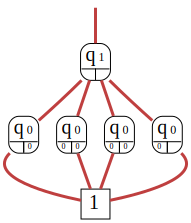
\includegraphics[width=8cm]{cnot.png}
        \end{subfigure}
        \hfill
        \begin{subfigure}{0.4\textwidth}
            \centering
            \includegraphics[width=3cm]{cnot_circuit.png}
        \end{subfigure}
        \caption{线性可逆电路可以用矩阵的行列变换表示}
    \end{figure}
    \begin{figure}
        \centering
        \includegraphics[width=4cm]{graph.png}
        \caption{如何在物理比特的连接性受限的约束下,减少cnot的数量是项目的重点}
    \end{figure}    
\end{frame}
\begin{frame}
    \frametitle{电路综合项目}
    \begin{figure}[htbp]
        \includegraphics[width=.8\textwidth]{phase.png}
        \caption{可以进一步推广线路可逆电路综合方法到phase network电路}
    \end{figure}
\end{frame}
\begin{frame}
    \frametitle{电路综合项目}
    \begin{figure}[htbp]
        \includegraphics[width=.8\textwidth]{dep.pdf}
        \caption{项目文件依赖图。其中绿色为测试文件,红色为外部库,黑色为项目文件。该项目中所有常数以及自定义类型在Config.hpp,项目中算法涉及的自定义类在typedef.hpp。}
    \end{figure}
\end{frame}
\begin{frame}
    \frametitle{密码项目-simon}
    \begin{figure}[htbp]
        \includegraphics[width=.8\textwidth]{simon.png}
        \caption{simon算法对于一个黑盒函数(black box)或oracle $f:\{0,1\}^n\to \{0,1\}^n$,已知存在一个比特串 $s, s\in \{0,1\}^n$ 使得对任意 $x,y\in\{0,1\}^n$,当且仅当 $x\oplus y\in \{0^n,s\}$时 $f(x) = f(y)$。问题的目标是使用尽可能少的查询或者调用函数,得到 $s$ 的值。}
    \end{figure}
\end{frame}

\begin{frame}
    \frametitle{密码项目-量子随机游走}
    \begin{figure}[htbp]
        \includegraphics[width=.8\textwidth]{qw.png}
        \caption{量子随机行走是经典随机行走的量子版,它在多边形上的应用包括图论、搜索算法和物理模拟等。量子游走可以分为离散时间量子游走和连续时间量子游走。离散时间量子游走(Discrete-Time Quantum Walk)的演化空间可记为:
        \(
        H = H_p \otimes H_c
        \)
        其中,\( H_p \) 是粒子游走的位置所张成的空间,\( H_c \) 是硬币态所张成的空间。对于一维量子游走,位置空间和硬币空间分别为:
        \(
        H_p = \text{span}\{ |x\rangle : x \in \mathbb{Z} \}, \quad H_c = \text{span}\{ |0\rangle, |1\rangle \}
        \)}
    \end{figure}
\end{frame}

% \begin{frame}
% \frametitle{Achievements and Recognition}
% \begin{itemize}
%     \item Award 1: [Description]
%     \item Recognition 1: [Description]
% \end{itemize}
% \end{frame}

\begin{frame}
\frametitle{其他项目与技能}
\begin{itemize}
    \setlength{\itemsep}{20pt}
    \item \textbf{VQE项目},用isq-python实现氢分子基态能量的计算
    \item \textbf{VHDL},实现过STM32架构下蓝牙模块与传感器的通信
    \item \textbf{COQ},完成过Softwarefoundation中卷一的逻辑命题的证明
\end{itemize}
\end{frame}

\begin{frame}
\begin{center}
    \huge
    谢谢各位!
\end{center}
\end{frame}

\end{document}
